\documentclass[12pt,french]{article}

\usepackage[utf8]{inputenc}
\usepackage[T1]{fontenc}
\usepackage{lmodern}
\usepackage[french]{babel}
\usepackage{graphicx,csquotes,textcomp}
\usepackage[titlepage,fancysections]{polytechnique}
\usepackage{url,menukeys}%Menukeys c'est pour les séquences de menu et les touches de clavier.
\usepackage[hidelinks]{hyperref}

\title{InfoBar}
\subtitle{Fonctionnement des bars d'étage\\Petit guide à l'utilisation de Chocapix}
\author{Par le BR 2013}
\date{Avril 2015}
\logo{logo}

\begin{document}

\maketitle

\section*{introduction}

\begin{center}
\bfseries Bienvenue sur le plâtal ! 
\end{center}

Ce guide a pour but d'expliquer le fonctionnement des bars d'étage à l'X et l'utilisation du logiciel Chocapix accessible sur \url{chocapix.binets.fr}\footnote{ou simplement \url{http://chocapix} si tout est bien configuré sur ton ordinateur.}. Si tu es respo bar et que tu cherches des conseils pour organiser la gestion de ton bar, va regarder les pages du WikiX idoines (\url{wikix.polytechnique.org/Respo_bar}).


\tableofcontents

\clearpage

\section{Le bar d'étage : comment ça marche ?}

\subsection{Une pièce polyvalente}

Il y a normalement un bar d'étage par section ; cependant, comme il n'existe que 14 bars d'étage pour 15 sections, il y a forcément un bar d'étage partagé entre deux sections. Mais ne t'inquiète pas ; plus on est de fous, plus on rit !

Le bar d'étage est le cœur de la vie de section, c'est là que tout le monde se retrouve après les cours, prend son goûter, regarde la télé, discute, se pose et surtout mange le soir ! Le Magnan est ouvert jusqu'à 19 h 15 le soir et tu peux y dîner mais c'est au bar d'étage que tu trouveras ta section et vivras de très bons moments.

Le bar d'étage est équipé d'une cuisine, profites-en pour te mettre à la gastronomie et préparer de bons petits plats le soir pour plusieurs, ton estomac et ta section te remercieront ! 

\subsection{Comment s'approvisionner ?}

Cela fait longtemps que les bars d'étage existent à l'X, et au fil des ans une forme d'organisation spécifique s'est développée. Le système est un peu compliqué mais le résultat en vaut la peine, donc lis attentivement les lignes suivantes pour comprendre comment ça marche !

Pour que les bars d'étage soient remplis de victuailles en toute circonstance, il est nécessaire de faire les courses (ou \enquote{faire une appro}) au moins une fois par semaine. Pour cela, la solution la plus pratique adoptée par tous les bars d'étage est de se faire livrer au pied des bâtiments par les services de \emph{drive} des supermarchés des environs.

Pour minimiser le nombre d'appros par semaine, il est donc logique que la section fasse des commandes groupées plutôt que chacun commande sa nourriture. Cette mutualisation des commandes et donc de la nourriture a plusieurs conséquences :
\begin{itemize}
	\item tout le monde doit venir aider pour monter et ranger l'appro ;
	\item il est plus facile de faire des plats à plusieurs ;
	\item il faut une équipe de gens motivés pour gérer tout ça.
\end{itemize}

Ces gens motivés, ce sont les respos bar, mais attention, cela ne veut pas dire qu'ils doivent tout faire dans le bar ! Tout le monde est concerné, et tu verras rapidement que l'état général d'une pièce mise en commun a une forte tendance à la dégradation fulgurante si tout le monde ne fait pas attention.

\subsection{Comment payer ?}

Avec la mutualisation de la nourriture, il y a \emph{a priori} plusieurs solutions pour partager les dépenses. La plus simple serait de faire payer chaque appro équitablement par tous les membres de la section. Mais un système plus sophistiqué et plus juste a été adopté, parce que chacun n'utilise pas le bar d'étage de la même manière. En voici le principe :
\begin{itemize}
	\item tout repose sur le logiciel bar appelé \enquote{Chocapix}, chaque utilisateur du bar y possède un \enquote{compte bar} qu'il approvisionne en faisant des chèques sur le compte du bar d'étage ouvert par les respos bar ;
	\item à chaque appro, les respos bar rentrent tous (ou presque) les aliments achetés dans le logiciel bar, avec les quantités et les prix ;
	\item à chaque fois que tu consommes quelque chose, tu dois le signaler en le rentrant dans le logiciel (sur l'ordinateur du bar ou dans ton casert) qui te débite de ton compte bar une somme d'argent égale au prix de ce que tu as consommé.
\end{itemize}

Ce système d'argent virtuel a plusieurs avantages : cela facilite les échanges d'argent entre membres d'une même section, permet d'économiser la petite monnaie pour les lessives, et théoriquement fait payer les gens pour ce qu'ils consomment réellement. 

Néanmoins, il y a des inconvénients, tous liés à la déviation du modèle à la réalité : il est très facile d'oublier de logguer ce qu'on a mangé, même avec un ordinateur dans le bar d'étage. Ce qui n'est pas loggué n'est pas débité sur ton compte bar mais représente un trou dans les finances du bar d'étage. Ainsi régulièrement les respos bar font le point sur la comptabilité et décident de renflouer les caisses soit par des amendes, soit par un appel aux dons, soit par une taxe collective car il faut qu'il y ait de l'argent sur le compte du bar à la banque pour pouvoir payer les appros.

\subsection{La propreté}

C'est un point très important : le bar d'étage va se salir très vite et le comportement naturel des gens est de ne pas s'en soucier. Et tout le monde doit participer à la propreté du bar d'étage ! Concrètement, il faut tous les soirs :
\begin{itemize}
	\item faire sa vaisselle et la ranger dans les endroits qui vont bien ;
	\item nettoyer la table où l'on a mangé ;
	\item jeter les bouteilles de bière, emballages, bouchons que l'on a laissés traîner ;
	\item enfin, en faire un petit peu plus que juste son petit coin parce que ça arrive à tout le monde d'oublier de nettoyer quelque chose.
\end{itemize}
Un conseil : si vous mangez à plusieurs, faites votre vaisselle et votre nettoyage à plusieurs, ça va plus vite et normalement ça prend 10 minutes pour faire la vaisselle et rendre tout propre derrière soi. Si vous faites ça, les respos bar vous en seront reconnaissants et n'auront pas à vous fister avec des amendes ou des nettoyages collectifs par la suite.

Des conseils pour maintenir un bar d'étage propre sont indiqués sur le WikiX à la page \url{http://wikix.polytechnique.org/Respo_bar/Respo_propreté}.

\clearpage

\section{Chocapix : côté utilisateur}

\subsection{Connexion}

\begin{figure}[h]
\centering
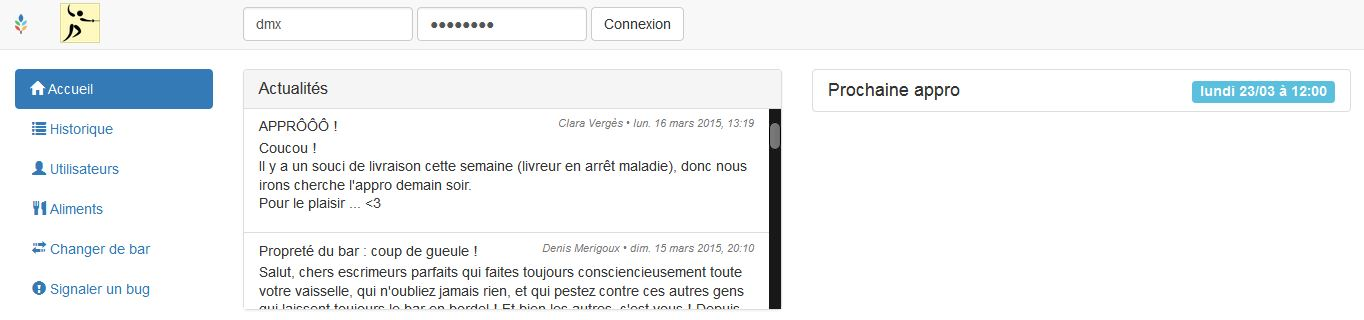
\includegraphics[width=16cm]{images/login}
\caption{Page de connexion}
\end{figure}

\paragraph{Se connecter} Si tu as un compte Frankiz, alors un compte Chocapix te sera créé automatiquement avec les informations suivantes :
\begin{description}
\item[Login] \texttt{prenom.nom} (le login de la DSI) ;
\item[Mot de passe] \texttt{0000}, mot de passe qu'il te faudra changer au plus vite.
\end{description}
Si tu n'as pas de compte Frankiz à ton arrivée sur le plâtal, demande à un des respos bar de ta section de créer ton compte.

Un fois connecté, tu arrives sur la page d'accueil du logiciel qui devrait te suffire pour logguer et t'informer sur ton bar d'étage. Tu y trouveras :
\begin{itemize}
	\item la MagicBar\texttrademark{} que tu utilises pour toutes les opérations ;
	\item la petite icône chariot à gauche de ton nom pour lancer une bouffe à plusieurs ;
	\item en haut à droite, ton solde et le bouton de déconnexion ;
	\item un panneau \menu{Actualités} au centre gauche qui affiche des messages écrits par les respos bar de ta section ;
	\item  à droite, la date de la prochaine appro et un rappel pour réapprovisionner ton compte lorsque le solde est faible ;
	\item en dessous, ton historique de consommation personnel avec tout ce que tu as acheté, les dépenses communes qui t'ont été prélevées, les dons, etc. ;
	\item à gauche, une colonne de navigation te permet d'accéder aux autres pages du site.
\end{itemize}

\begin{figure}[h]
\centering
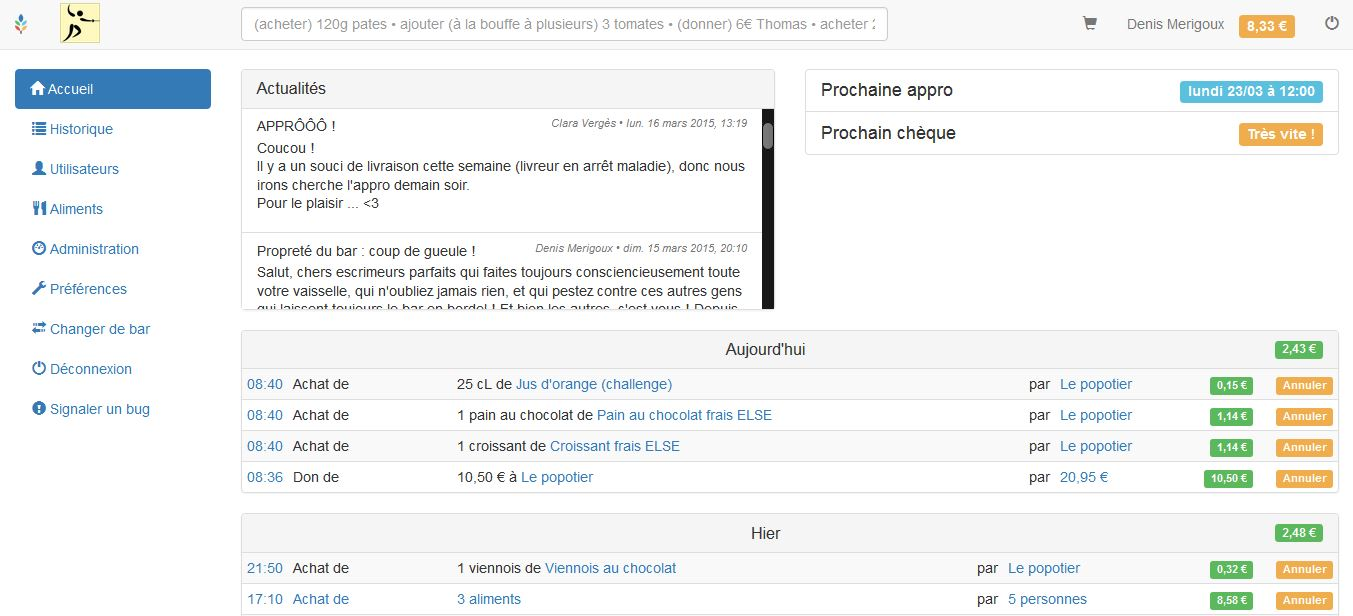
\includegraphics[width=16cm]{images/home}
\caption{Page d'accueil de Chocapix\label{home}}
\end{figure}

\paragraph{Se déconnecter} Appuie sur le bouton \menu{Déconnexion} en forme de bouton power en haut à droite ou tape deux fois \keys{Echap} (attention, raccourci extrêmement nuisible).

\subsection{Logguer}

\paragraph{Pour soi-même} Grâce à la MagicBar\texttrademark{}, il est très simple de logguer tes aliments sur le site : il suffit de rentrer les premières lettres du nom de l'aliment puis la quantité (en unités définies à l'avance par les respos bar), de sélectionner le bon aliment dans le menu déroulant à l'aide des flèches directionnelles \keys{$\uparrow$} et \keys{$\downarrow$} du clavier, appuyer sur \keys{Entrée} et c'est bon !

Il y a d'autres manières de réaliser la même opération, en gros tu peux rentrer à peu près n'importe quoi qui aie du sens et la MagicBar\texttrademark{} l'interprètera correctement. D'ailleurs des exemples de syntaxe sont marqués en gris dans le champ de texte lorsque tu n'y as rien entré.

\begin{figure}[h]
\centering
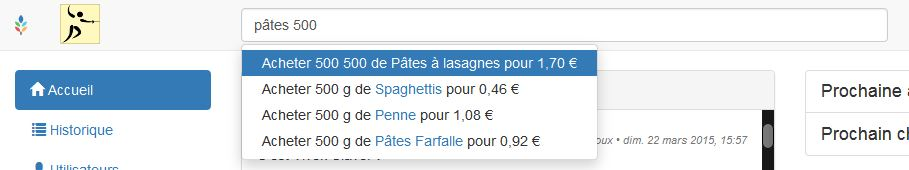
\includegraphics[width=16cm]{images/log}
\caption{MagicBar\texttrademark{} : logguer un aliment.}
\end{figure}


\paragraph{Bouffe à plusieurs} Il arrivera fréquemment que tu prépares un repas pour plusieurs personnes, dont il faudra diviser le prix entre les participants. Il y a un outil adapté à cela dans Chocapix, la bouffe à plusieurs :
\begin{enumerate}
	\item avant de rentrer les ingrédients, clique sur le petit chariot en haut à droite ;
	\item entre le nom du plat ou de la bouffe ;
	\item ajoute les participants en tapant dans le champ les premières lettres de leur nom ou prénom puis en appuyant sur \keys{Entrée}, tu peux régler la part de ce qu'ils payent à côté de leur nom ;
	\item entre les ingrédients de la bouffe à plusieurs dans la MagicBar\texttrademark{} comme si tu les logguais tout seul ;
	\item lorsque tu as fini, clique sur \menu{Valider}.
\end{enumerate}
Tu peux aussi démarrer une bouffe à plusieurs en tapant « Ajouter » devant le nom de ton premier ingrédient dans la MagicBar\texttrademark{}.

\begin{figure}[h]
\centering
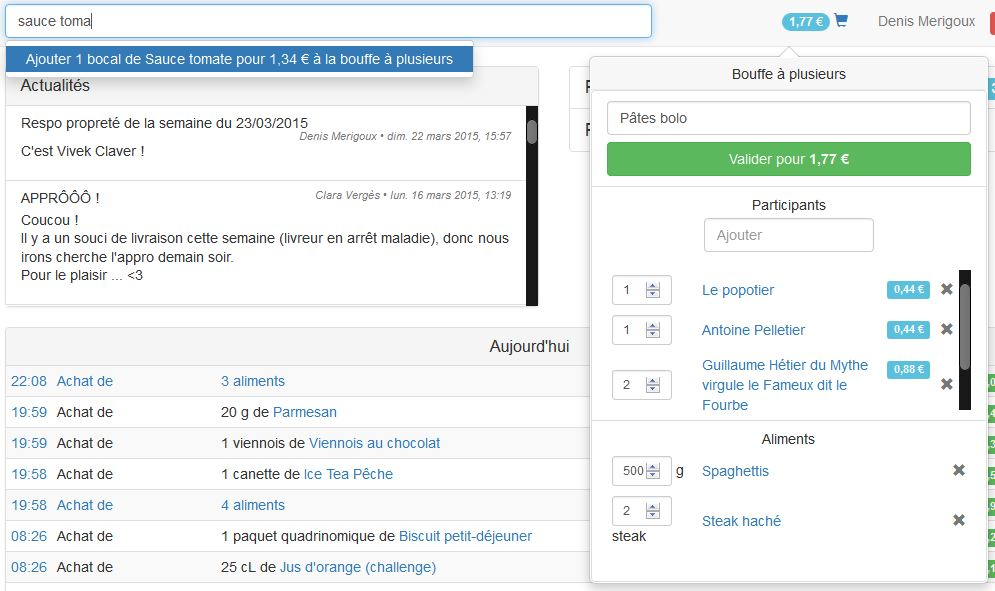
\includegraphics[width=16cm]{images/bouffeaplusieurs}
\caption{Faire une bouffe à plusieurs}
\end{figure}

\subsection{Compte personnel}

\paragraph{Situation personnelle} Tu peux voir tes données personnelles et ton historique de consommation en cliquant sur ton nom en haut à droite.

\paragraph{Préférences} Dans le menu \menu{Préférences} accessible depuis l'onglet de droite, tu pourras modifier ton login, ton pseudo et ton mot de passe (à faire au début pour changer du 0000 initial !).

\begin{figure}[h]
\centering
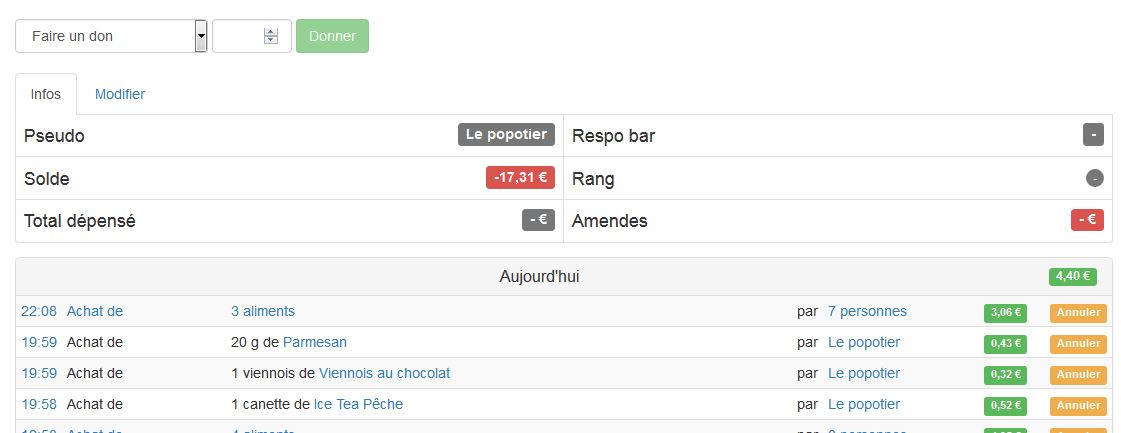
\includegraphics[width=16cm]{images/infosperso}
\caption{Informations et historique personnel}
\end{figure}

\subsection{Utilisateurs, aliments, historique, changement de bar et bugs}

\paragraph{Autres utilisateurs, dons} Dans le menu \menu{Utilisateurs} à gauche, tu pourras trouver la liste des utilisateurs de ton bar. Si tu cliques sur un nom, tu accèderas à ses informations personnelles et tu pourras lui faire un don en entrant le montant et en cliquant sur \menu{Donner}.

\paragraph{Aliments, opérations} Dans le menu \menu{Aliments} à gauche tu trouveras la liste des aliments vendus par ton bar avec la quantité théorique restante (négative si tes respos bar n'ont pas encore entré l'appro ou si les gens ont trop loggué l'aliment) et le prix par unité.

En cliquant sur le menu déroulant en dessous du nom de l'aliment, tu peux acheter l'aliment pour toi, le mettre dans une bouffe à plusieurs ou déclarer la quantité d'aliments que tu jettes à la poubelle (s'ils sont périmés par exemple). Dans ce dernier cas, tu ne paieras pas ce que tu jettes mais ça permet aux respos bar de mieux gérer les stocks.

\paragraph{Changer de bar} En cliquant \menu{Changer de bar} à gauche, tu pourras accéder aux pages des autres bars d'étage, et y logguer des aliments si tu y possèdes un compte. \textbf{Attention} : tu possèdes un solde bar par bar d'étage, et non pas un solde unique pour tous les bars où tu es inscrit. En effet, l'argent qui est virtuellement sur ton solde bar est réellement sur le compte en banque du bar d'étage, donc on ne peut pas rassembler virtuellement l'argent qui est réellement sur plusieurs comptes en banque.

\paragraph{Signaler un bug} En cliquant sur \menu{Signaler un bug}, tu peux envoyer un message à l'équipe de développement de Chocapix qui s'empressera de corriger l'erreur si jamais tu donnes des informations assez précises sur l'emplacement du bug. Utilise cette fonction pour que le site bar soit encore mieux !


\section{Chocapix : côté respo bar}

Si tu viens d'arriver sur le plâtal, va voir sur le WikiX à la page \url{http://wikix.polytechnique.org/Respo_bar/Arrivée} ; tu y trouveras des conseils et la marche à suivre pour démarrer ton bar d'étage.

\subsection{Respo bar}

\subsubsection{Les droits utilisateurs}

Certains membres de la section, les respos bars, ont accès à des fonctionnalités supplémentaires sur le site, toutes accessibles depuis l'onglet \menu{Administration} à gauche. Au début, un respo bar administrateur est promu en tant que tel par les administrateurs de Chocapix : pour cela il suffit d'envoyer un mail à \href{mailto:babe@eleves.polytechnique.fr}{\texttt{babe@eleves.polytechnique.fr}} pour signaler qui sera ce respo bar pour ta section. Ce respo bar tout-puissant pourra ensuite déléguer des droits à d'autres membres de la section pour gérer chaque aspect de l'administration de son bar d'étage via Chocapix :
\begin{itemize}
	\item les respos bar ont accès à toutes les fonctionnalités ;
	\item le respo appro aura globalement accès au menu \menu{Administration>Aliments} ;
	\item le respo inventaire pourra faire un inventaire dans \menu{Administration>Aliments>Faire un inventaire} ;
	\item le respo news aura accès au menu \menu{Administration>Actualités} ;
	\item le trézobar aura accès au menu \menu{Administration>Comptabilité} et pourra modifier le solde des utilisateurs ;
	\item le respo amendes pourra mettre des amendes.
\end{itemize}
Il est possible de cumuler les postes ou de les doublonner. Il est d'ailleurs conseillé de donner les droits à plusieurs personnes pour qu'il y ait toujours quelqu'un disponible pour logguer une appro, par exemple.

\subsubsection{Droits spécifiques au respos bar}

\paragraph{Modifications des droits utilisateur} Dans le menu \menu{Utilisateurs>(Nom de l'utilisateur)>Modifier} tu pourras rajouter ou enlever des droits d'administration selon les principes de la section précédente.

\paragraph{Création d'un compte} Dans le menu \menu{Administration>Utilisateurs>Créer un utilisateur}, tu peux créer le compte d'un nouvel utilisateur de ton bar d'étage. Rentre bien toutes les informations comme il faut, car le nom ou le prénom ne pourront pas être changés par la suite.

\subsection{Respo appro}

Des conseils généraux pour les respos appro et un comparatif des différents supermarchés sont indiqués sur le WikiX à la page \url{http://wikix.polytechnique.org/Respo_bar/Respo_appro}.

Comme expliqué par la suite, le système des aliments repose sur les codes-barres des produits achetés. Il est donc très fortement conseillé d'acheter pour ton bar d'étage un lecteur de codes-barres USB. Cela coûte 20 € et s'utilise sans installer de logiciel sur n'importe quel ordinateur. Le principe est simple : à chaque fois que tu scannes un code-barres, un bip retentit et sur l'ordinateur tout ce passe comme si tu avais rentré le code-barres au clavier et appuyer sur \keys{Entrée}. Pour te donner un exemple de quoi commander, voici ce qu'ont commandé et testé avec succès les deux bars d'étage de test : \url{http://www.amazon.fr/Tera%C2%AE-scanner-barre-Lecteur-poche/dp/B009IF1DYK/}.

\subsubsection{Système des aliments dans Chocapix}

Avant d'expliquer comment logguer une appro, il faut commencer par expliquer comment sont modélisés les aliments dans Chocapix. Chaque produit acheté est unique et identifié par son code-barres ; quand un respo bar loggue pour la première fois un aliment inconnu de Chocapix, la correspondance entre code-barres et aliment est inscrite dans une base de données commune à tous les bars d'étage. Donc un produit acheté sur la facture de ton appro égale un produit dans la base de données de produits achetés de Chocapix.

Mais il existe un deuxième type d'aliments, les aliments vendus par ton bar. En effet, pour éviter d'avoir 250 aliments à vendre dans ton bar avec la confusion que ça peut entraîner pour les consommateurs, tu vas sans doute préférer regrouper les yaourts goût fraise avec ceux goût framboise... Donc les produits que ton bar vendra aux consommateurs regroupent un ou plusieurs aliments achetés ; le prix de l'aliment vendu est calculé comme la moyenne des prix des produits achetés qui le compose, pondérés par les quantités desdits aliments. Pour faire simple, une fois que tout ton aliment vendu aura été loggué, cela correspondra exactement à la somme des prix des aliments achetés correspondants.

Enfin, il y a certains aliments que ton bar ne fera pas payer et dits \enquote{en open} : l'huile, le sel, le beurre, etc. C'est toi qui choisis ce que tu fais payer ou pas, mais cela ne sert à rien de rentrer dans le logiciel le détail exact des produits en open. Par contre, ils seront pris en compte dans la comptabilité comme expliqué plus loin.

Compliqué ? Un peu, mais quand tu comprendras un peu mieux la problématique de la gestion des aliments dans un bar d'étage tu t'apercevras que c'est une solution tout à fait viable, et meilleure que celle qui existait dans l'ancien site bar.

\subsubsection{Ajouter un aliment à la vente\label{ajout}}

Avant de pouvoir rentrer une appro dans Chocapix, il faut d'abord créer les aliments que ton bar vendra. Pour cela, va dans \menu{Administration>Aliments>Ajouter un aliment} et suis les étapes suivantes :
\begin{enumerate}
	\item scanne le code-barres du nouvel aliment ou rentre-le à la main\footnote{taper un code-barres à la main, c'est subaïsse (voir le WikiX pour l'étymologie de ce terme), d'où l'utilité du scanner de codes-barres...} et appuie sur \keys{Entrée} ;
	\item si le code-barres n'est pas dans la base de données, rentre dans le champ \menu{Nom d'achat} le nom exact de l'aliment, du type \texttt{Type\_aliment Marque Contenant Quantité Unité} et son pluriel ; si le code-barre est déjà dans la base de données, les champs se rempliront tous seuls et tu ne pourras pas les modifier ;
	\item la section du dessous concerne la correspondance entre produit acheté et aliment vendu ; soit tu crées un nouvel aliment vendu en remplissant les champs correspondants (et notamment la conversion entre un produit acheté et le nombre d'unités d'aliment vendu auquel cela correspond), soit tu rattaches ce produit acheté à un aliment déjà vendu par le bar (tape les premières lettres de l'aliment vendu dans le champ \menu{Aliment} et tu le verras apparaître), regroupant ainsi plusieurs produits achetés pour un seul aliment vendu.
\end{enumerate}
Si tu crées un nouvel aliment vendu, tu devras aussi définir la taxe appliquée à cet aliment. La taxe couvre les vols ou oublis de log (il y en aura) et le prix des produits en open que propose ton bar d'étage. Il est par expérience conseillé de fixer cette taxe à 20 \% pour tous les produits, mais là encore c'est toi qui choisis.

\paragraph{Aliments simples et packs} Il y a des aliments qui ne portent pas de code-barres ; tu peux quand même les ajouter, en laissant vide le champ du code-barres. Ces aliments ne seront néanmoins pas ajoutés à la base de données inter-bars. Par contre il y a des aliments vendus en packs qui eux portent un code-barres. Dans ce cas, tu dois rentrer le produit acheté comme unité d'abord puis entrer le code-barres du pack, sélectionner \menu{Il s'agit d'un pack} et remplir les champs comme il faut.


\subsubsection{Rentrer une appro}

\paragraph{Méthodologie} Tu as deux solutions pour logguer une appro : en même temps que tu ranges les aliments ou bien plus tard, au calme, dans ton casert si tu préfères.

Pas besoin de la rentrer immédiatement après avoir rangé les aliments dans les armoires, tu peux attendre une demi-journée voire plus : les gens peuvent logguer des aliments même si la quantité théorique restante est négative. Par contre pour la première appro et pour les nouveaux aliments, il faut les rentrer le plus vite possible dans le logiciel pour que les gens puissent les logguer.

Pour rentrer une appro, prends ta facture, va dans \menu{Administration>Aliments>Faire une appro} et suis les étapes suivantes pour chaque item de la facture :
\begin{enumerate}
	\item si ta facture affiche les codes-barres des aliments, scanne-les, sinon entre les premières lettres du produit acheté dans le champ \menu{Ajouter} et appuie sur \keys{Entrée} ;
	\item appuie sur \keys{Tab} pour sélectionner le champ \menu{Quantité}, et entre la quantité achetée au clavier, puis rappuie sur \keys{Tab} pour modifier le prix total d'achat pour cet aliment si nécessaire ;
	\item appuie une ou deux fois sur \keys{Shift+Tab} pour revenir au champ \menu{Ajouter} et recommence.
\end{enumerate}
Tu peux logguer une appro sans te servir de la souris ! Sers-toi des raccourcis clavier, tu iras beaucoup plus vite. Tu remarqueras que Chocapix te propose de logguer les produits achetés à l'unité ou en packs si tu as bien rentré les packs.

Une fois que tu as ajouté tous les aliments de la facture (sauf les produits en open ou le matériel payé en commun), note (ou demande au trézobar de le faire) dans \menu{Administration>Comptabilité>Loguer du matériel} la somme des prix de tous les produits en open. Cette somme d'argent ne sera pas débitée sur les comptes bar mais rentrera comme une dépense sur la comptabilité du site.

Tu peux aussi faire payer les produits en open à tout le monde en entrant un paiment collectif dans \menu{Administration>Utilisateurs>Paiement collectif}.

\subsubsection{Opérations sur les aliments}

Une fois l'appro rentrée, tu auras sûrement besoin de modifier les informations des aliments et les quantités des stocks.

\paragraph{Aliments vendus} Tu peux modifier les informations relatives à un aliment vendu par ton bar en allant dans \menu{Aliments>(Nom de l'aliment)>Modifier}. Notamment tu peux décider de changer l'unité de vente de ton aliment (passer du nombre au poids par exemple). Pour cela, modifie le champ \menu{Unité de vente}, des champs supplémentaires apparaîtront et te permettront de faire le changement sans problème.

Dans l'onglet \menu{Stocks}, tu peux modifier les quantités et les prix des différents produits achetés qui sont regroupés dans ton aliment vendu afin de jouer sur le prix et la quantité de ton aliment vendu.

\paragraph{Produits achetés} Tu peux accéder à la liste des produits achetés par ton bar dans \menu{Administration>Aliments>Liste des aliments}. La liste affiche la quantité restante théorique de chaque produit acheté et le prix d'achat d'une unité de cet aliment. Néanmoins tu ne peux pas modifier toi-même les informations relatives à un produit acheté comme le nom du produit acheté. Ces informations sont entrées une fois pour toutes lors de l'ajout initial du produit acheté dans la base de données. Néanmoins tu peux envoyer un mail à \href{mailto:babe@eleves.polytechnique.fr}{\texttt{babe@eleves.polytechnique.fr}} pour indiquer que tu souhaites un changement.

\paragraph{Regrouper des articles} Dans \menu{Administration>Aliment>Regrouper des articles}, tu peux fusionner deux aliments vendus par le bar en un seul : cela regroupera les produits achetés correspondants. Pour enlever un produit acheté d'un aliment vendu, c'est \menu{Aliments>(Nom de l'aliment)>Sotcks>Retirer}. Pour ajouter un produit acheté à un aliment vendu, c'est \menu{Administration>Aliments>Ajouter un nouvel aliment>Rattacher à un aliment déjà vendu}.

\subsection{Respo inventaire}

Pour que les quantités affichées sur Chocapix soient reliées à la réalité et te rendre compte de l'ampleur des vols, il te faudra régulièrement (une fois par mois environ) faire un inventaire de tout ce que contient ton bar. Fais-le la veille d'une appro, il y a moins de boulot à faire.

Pour cela, va dans \menu{Administration>Aliments>Faire un inventaire} et rentre un à un les produits achetés présents dans ton bar d'étage en scannant leur code-barres ou en recherchant leur nom.

Tu as aussi accès à \menu{Administration>Aliments>Ajouter une aliment}, au cas où il y aurait un aliment non répertorié dans ton inventaire. Regarde la section \ref{ajout} pour savoir comment faire.

\subsection{Respo news}

Le respo news est chargé de la communication des respos bars aux autre membres de la section. Cela peut se faire par mail section mais Chocapix offre plusieurs possibilités pour informer les gens sans les spammer.

\paragraph{Prochaine appro} Dans \menu{Administration>Actualités>Annoncer la prochaine appro}, tu peux définir la date de la prochaine appro, qui sera visible par tout le monde sur la page d'accueil de Chocapix. N'oublie pas de la changer après chaque appro !

\paragraph{Actualités} Une actualité est un petit texte avec un titre qui est affiché sur la page d'accueil de ton bar d'étage sur Chocapix. Ces messages peuvent être très divers : annonce du respo propreté, d'une appro spéciale, d'un repas section, etc. Pour ajouter une annonce, c'est \menu{Administration>Actualités>Ajouter une news}. Pour afficher toutes les news ou les modifier, c'est \menu{Administration>Actualités>Lister les news}. Tu peux notamment faire remonter une news pour qu'elle s'affiche en premier.

Les news publiées ou modifiées depuis moins d'un jour sont affichées en bleu sur la page d'accueil, elles deviennent ensuite blanches.

\subsection{Trézobar}

Le trésorier du bar gère la trésorerie du bar, qui est un peu subtile. Tout est détaillé sur le WikiX à la page \url{http://wikix.polytechnique.org/Respo_bar/Trézobar}. Chocapix peut gérer presque tous les aspects de la trésorerie du bar, et t'indiquer si ton bar est en déficit ou en positif via l'indicateur de la page d'accueil de l'onglet \menu{Administration}.

\paragraph{Appro} Lors d'une appro, il faut veiller à ce que le respo appro rentre dans le logiciel :
\begin{itemize}
	\item tous les produits vendus par le bar au bon prix ;
	\item le montant des produits en open.
\end{itemize}
Ainsi l'indicateur \enquote{sur le compte bancaire du bar (théorique)} \menu{Administration>Comptabilité>État du bar} est bien débité de la valeur exacte de ce que tu as payé au supermarché.

\paragraph{Matériel et dépenses communes} Lorsque tu engages une dépense commune comme l'achat de matériel ou l'organisation d'une bouffe section, il y a deux choses à faire :
\begin{enumerate}
	\item indiquer la somme exacte dépensée dans \menu{Administration>Comptabilité>Logguer du matériel} ;
	\item faire payer la somme par les membres de la section dans \menu{Administration>Utilisateurs>Paiement collectif}.
\end{enumerate}

\paragraph{Solde des utilisateurs} Chaque semaine, après avoir porté les chèques de tes camarades à la banque, il te faudra créditer leur compte de la somme correspondante en allant dans \menu{Utilisateurs>(Nom de l'utilisateur)}, en cliquant sur la flèche à côté de \enquote{Faire un don}, en sélectionnant \enquote{Créditer le compte}. Tu peux aussi sélectionner l'option \enquote{Rembourser une appro} pour mettre un motif et rembourser \emph{via} compte bar un membre de la section qui a avancé les frais pour une appro. Ces deux options rajoutent de l'argent sur le compte utilisateur mais n'en enlèvent pas sur l'indicateur du compte bancaire théorique du bar.

Les deux autres options \enquote{Retirer de l'argent} et \enquote{Mettre une amende} fonctionnent différemment. En effet, la première option est à utiliser lorsqu'un membre de la section veut récupérer de l'argent qui est sur son compte bar : l'argent retiré est retiré de l'indicateur compte bancaire du bar, car tu donnes physiquement un chèque à celui qui vient retirer son argent. Par contre, lorsque tu mets une amende, tu retires de l'argent virtuel à quelqu'un mais le compte en banque de ton bar n'en est pas affecté, donc l'indicateur restera inchangé.

\paragraph{Agios} Dans \menu{Administration>Paramètres}, tu peux régler l'indicateur de solde bas pour tous les utilisateurs du bar et aussi activer les agios pour inciter ceux qui ont des comptes en négatif à les approvisonner. Tu peux aussi définir le coefficient multiplicateur pour le calcul des agios, ainsi que le nombre de jours entre le passage en négatif et le déclenchement du premier agio.

%\paragraph{Dépenses et recettes} Tu peux afficher les dépenses et recettes pour le compte du bar d'étage dans \menu{Administration>Comptabilité>Compte bancaire}. Toutes ces dépenses et recettes doivent être celles qui sont marquées sur ton relevé de compte en ligne sur le site de ta banque, sauf les appros (qui sont gérées via l'appro d'aliments et le montant des produits en open) et les dépenses liées à ELSE (voir plus bas). Tu peux aussi rajouter manuellement une dépense ou une recette qui sort de l'ordinaire des appros : voyages section, activités cohésion, pulls section, etc.

\paragraph{ELSE} Si ton bar possède un compte chez ELSE, il y a une petite subtilité supplémentaire. En effet ton bar possède un solde chez ELSE, qui n'est pour l'instant pas géré par Chocapix. Ainsi il est conseillé de procéder comme il suit :
\begin{enumerate}
	\item à chaque appro ELSE, tu loggues les aliments achetés et le prix des aliments achetés est donc débité de l'indicateur compte bancaire du bar ;
	\item tu ne rentre pas dans le logiciel les chèques que tu fais à ELSE ;
	\item à chaque instant, la somme de ce qui est indiqué sur l'indicateur du compte bancaire théorique dans \menu{Administration>Comptabilité>État du bar} et du solde ELSE de ton bar doit être égale à ce qui apparaît sur le site Internet de la banque où ton bar a son compte.
\end{enumerate}

\paragraph{Conclusion} La comptabilité demande un peu de travail toutes les semaines, mais à part la manip' avec ELSE détaillée au dessus, ce que tu as sur le site de ta banque doit coïncider exactement avec l'indicateur du compte bancaire théorique dans \menu{Administration>Comptabilité>État du bar}. De cette manière, le logiciel peut en déduire l'état de tes finances et t'afficher le solde réel de la comptabilité de ton bar (calculé par la formule qui est sur le WikiX) sur l'écran d'accueil de l'onglet \menu{Administration}.




\end{document}